\documentclass[twocolumn]{article}
\usepackage{verbatim}
\usepackage{amsfonts}
\usepackage{geometry}
\usepackage{amsmath}
\usepackage{amsthm}
\usepackage{amssymb}
\usepackage{listings}
\usepackage{graphicx}
\usepackage{clrscode3e}
\usepackage{txfonts}
\usepackage{enumerate}
\usepackage{ctex}
\usepackage{txfonts}
\usepackage{fontspec-xetex}
\usepackage{float}
\geometry{top=2.5cm,bottom=2.5cm,left=2.5cm,right=2.5cm}
\setlength\parindent{0em}
\setmainfont{Times New Roman}
\newcommand*{\dif}{\mathop{}\!\mathrm{d}}
\begin{document}
	\title{问题求解(二)作业(第十三周)}\author{161180162 许致明}\maketitle
	\section*{TC第12章}
	\subsection*{12.1-2}
	BST: $x.left\leq x$ and $x.right>x$\par
	Minimum Heap: $x.left\geq x$ and $x.right\geq x$\par 
	It's not possible, since for a heap, its left child and right child's keys doesn't have any greater or less relationship. So only by traversing the heap for $O(n)$ time is unable to output all keys in order.
	\subsection*{12.1-5}
	\begin{proof}
		Building a BST using sorting algorithm based on comparing is just like sort these data. Since the lower bound of comparison-based sorting algorithm is $\Omega(nlgn)$, the lower bound of building a BST by comparison is also $\Omega(nlgn)$.
	\end{proof}
	\subsection*{12.2-5}
	\begin{proof}
		Denote this Node as x, then $x.left.key\leq x.key$ and $x.right.key\geq x.key$.\par
		\begin{enumerate}[a.]
		\item Suppose $S=SUCCESSOR(x)$, then if S.left exists, $S.left.key\leq S$, and S is located in x's right subtree. So $S.left.key\geq x.key$ and $S.left.key\leq S.key$, in this case, S.left is x's successor, which contradicts our assumption. As a result, x's successor doesn't have a left child.
		\item Suppose $P=PREDECESSOR(x)$, and P has a right child P.right. We have $P.key\leq x.key$ and $P.right.key\geq P.key$. Besides, P.right is located in x's left subtree. So $P.right.key\leq x.key$, in this case, P.right is the predecessor of x, which contradicts our assumption. Therefore, x's predecessor doesn't have a right child.
		\end{enumerate}
	\end{proof}
	\subsection*{12.2-9}
	\begin{proof}
		If x is the left child of y, then $x.key<y.key$ and $y.right.key>y.key>x.key$.
		For since $x$ is the left child of $y$, all decedents in $y$'s right subtree is larger than $x$ and $y$. So $y.key$ is the least key that is larger than $x.key$. Similarly, if $x$ is the right child of $y$, $y.key$ is the largest key that is less than $x.key$.
	\end{proof}
	\subsection*{12.3-5}
	\begin{codebox}
		\zi\proc{Tree-Insert(\id{y}, \id{x}, \id{x})}\li 
		\If $x\neq NIL$\Then\li 
		\If $z.key<x.key$ \Then\li 
		\proc{Tree-Insert(\id{x}, \id{x.left}, \id{z})}\li 
		\Else\li 
		\proc{Tree-Insert(\id{x}, \id{x.right}, \id{z})}\End\End\li 
		\If $y==NIL$\Then\li
		$T.root=y$\li 
		\ElseIf $z.key<y.key$\Then\li 
		$y.left=z$\li 
		$x.suce=y$\li 
		\Else \li 
		$y.right=z$\li 
		$z.suce=y.suce$\li 
		$y.suce=z$\End
	\end{codebox}
	\begin{codebox}
		\zi\proc{Tree-Pred(\id{x}, \id{k})}\li 
		\If $k<x.key$\Then\li 
		$y=x.left$\li 
		\Else \li 
		$y=x.right$\End\li
		\If $y==NIL$\Then\li 
		raise error\li 
		\ElseIf $y.key==k$\Then\li 
		\Return $x$\li 
		\Else\li 
		\Return \proc{Tree-Pred(\id{y}, \id{k})}\End  
	\end{codebox}
	\section*{TC第13章}
	\subsection*{13.1-5}
	\begin{proof}
		Since this tree has a certain number of black node along every way downwards, the shortest way's length is the number of black nodes. According to the theorem, red nodes can't be adjacent, and red node's child must be black, the longest is that black and red nodes come up one after another. That is twice the number of the certain number black number has along one way downwards. So the longest way is at most twice the length of the shortest one.
	\end{proof}
	\subsection*{13.1-7}
	If black and red nodes come up one after another, and all nodes at bottom is red, the ratio at most is 2:1. If all this tree's nodes is black, the ratio at least is 0.
	\subsection*{13.2-2}
	\begin{proof}
		There are n nodes, then there are n-1 sides, every side can be rotated left or right, so there are n-1 possible ways of rotation.
	\end{proof}
	\subsection*{13.3-1}
	If that node is black, then the fifth property of a RB Tree is violated, making it much more difficult to adjust.
	\subsection*{13.3-5}
	\begin{proof}
		If an insertion doesn't violate any property of a RB Tree, it's obvious that this node is red. Then suppose the worst case, all of the n-1 nodes are adjusted and made black. Wherever the last node is inserted, since it's first made red, it won't violate any property. So the last node must be red. Therefore, there is at least one red node.
	\end{proof}
	\subsection*{13.4-1}
	\begin{proof}
		If x is the root, then it will be made black.If x is red and is not root, the loop won't take effect, and the root remains black. If x is black and is not root, then the program will enter the loop. x.p will be made red(see line 6). After case 1, it will enter case 2, 3, 4. In case 2, x.p is the new x node and made red. Loop terminates. At last x is made black. If entering case 3, 4, (see line 18)x.p is made black, if x.p is root, it remains black. If it directly enters case 2, then x.p is replaced by x. If the new x is red, loop terminates, at last it is made black. If it directly enters case 3, 4, if x.p is root, it will made black in line 18, then in case terminates. After all, the root is still black.
	\end{proof}
	\subsection*{13.4-7}
	Not the same. An example is shown below.
	\begin{figure}[H]
		\centering
		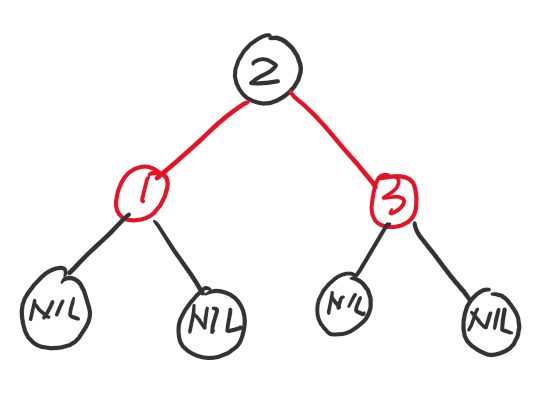
\includegraphics[width=0.7\linewidth]{13-1}
		\caption{插入顺序为3,2,1}
	\end{figure}
		\begin{figure}[H]
			\centering
			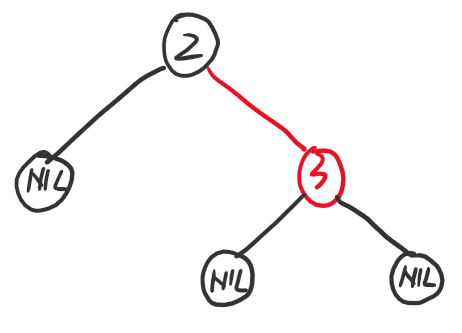
\includegraphics[width=0.7\linewidth]{13-2}
			\caption{删去节点1}
		\end{figure}
	\begin{figure}[H]
		\centering
		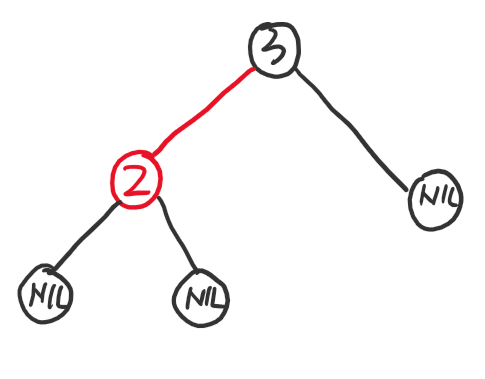
\includegraphics[width=0.7\linewidth]{13-3}
		\caption{插入顺序为1,3,2时,删去1}
	\end{figure}
	Obviously, Fig 3 is different from Fig 2.
\end{document}